\documentclass[main.tex]{subfiles}
\begin{document}

\chapter{Introduction}
The main topic of the thesis and the motivation behind it are introduced in this chapter.
It starts with a presentation of the problem background in \Cref{sec:background} followed by the purpose of the thesis in \Cref{sec:purpose}.

\section{Background}%
\label{sec:background}
In this section the problem background of the thesis is presented.
First, the motivation for quantum computing will be briefly presented.
Then a quick introduction to quantum error correction is given followed by the theory behind the \emph{cat code}.
After that the theory behind superconducting resonators and qubits will be reviewed in order to understand the cat code encoding scheme, where the latter will finally lead into the concept of quantum optimal control.
The reader will be assumed to have basic knowledge of quantum mechanics, quantum computing and quantum optics (specifically coherent states and the Wigner function).

\subsection{Potential of Quantum Computing}
Quantum computers are thought to solve problems which are not possible with classical computers~\cite{preskill_quantum_2018}.
Perhaps the most famous example is using \emph{Shor's algorithm} for prime factorization~\cite{shor_polynomial-time_1997} which could break some public key cryptographic algorithms.
Aside from quantum algorithms, there is also the prospect of using quantum computers to simulate quantum systems, which Feynman famously proposed~\cite{feynman_simulating_1982} back in 1982.
Since quantum systems form the basis of chemistry, particle physics and condensed matter physics, to name a few, we hope that quantum simulation can help these sciences with discoveries such as new medicine, collider dynamics and materials.  

While quantum computers are starting to appear as commercial products~\cite{santos_ibm_2016}, there are still a lot of challenges to be solved before large scale quantum computers can become commonplace.

\subsection{Quantum Error Correction}
One of the main challenges in building a quantum computer is combating decoherence, the process in which the quantum information of a quantum system leaks out into the environment~\cite{gottesman_introduction_2009}.
To solve this one can perform quantum error correction (QEC).
This can be done by introducing redundancy into the physical system and ``spread'' the quantum information to highly entangled states using quantum error correcting codes (QECC)~\cite{gottesman_introduction_2009}.
The two prevailing methods are to either (1) encode a logical qubit into many physical qubits, or (2) encode a logical qubit into a bosonic mode in quantum harmonic resonators~\cite{}.
Method (2) permits us to use a single physical system to store the information, which makes it a good candidate for a QECC.
\citeauthor{leghtas_hardware-efficient_2013}~\cite{leghtas_hardware-efficient_2013},~\citeauthor{mirrahimi_dynamically_2014}~\cite{mirrahimi_dynamically_2014} propose and~\citeauthor{ofek_extending_2016}~\cite{ofek_extending_2016} demonstrate a QECC called the ``cat code'', which will be the focus of this thesis.
The motivation for using the cat code for QEC is that the logical basis states are eigenstates of photon-number parity, which means that the cat code requires just a single ancilla qubit in order to monitor the dominant
error in the resonator (single photon loss)~\cite{ofek_extending_2016}.

\subsection{Cat Code}%
\label{sec:cat-code}
The logical basis states of the cat code
\begin{equation}
    \ket{0_L} = \cat{},\quad \ket{1_L} = \cat[i]{}
\end{equation}
are built up of \emph{cat states}: superpositions of coherent states
\begin{equation}
	\cat[]{} = \frac{1}{\sqrt{2}}\qty(\ket{\alpha} + \ket{-\alpha}),\quad 
	\cat[i]{} = \frac{1}{\sqrt{2}}\qty(\ket{i\alpha} + \ket{-i\alpha}).
\end{equation}
That is each basis state \( \ket{0(1)_L} \) in the cat code consists of a cat state \(\cat[(i)]{}\), which is a superposition of a coherent state \(\ket{(i)\alpha}\) and its negative counterpart \(\ket{-(i)\alpha}\). \(|\alpha|^2\) is the mean photon number of the coherent state.
%A coherent state can be represented in the Fock basis as
%\begin{equation}
%    \ket{(i)\alpha} =\ex^{-{\frac{|(i)\alpha|^2}{2}}}\sum_{n=0}^{\infty}{\frac{\qty((i)\alpha)^n}{\sqrt{n!}}}\ket{n}.
%\end{equation}
The basis can also be in an odd parity where the two coherent states are subtracted instead of added, however only the even parity basis will be used in this thesis for simplicity.

These basis states can be visualized by plotting the Wigner function which is done in \Cref{fig:cat-code-basis-wigner}. The characteristic features of a cat state in the Wigner plot are two lobes with interference fringes in between them~\cite{girvin_schrodinger_2017}.

\begin{figure}[H]
	\centering
	\subcaptionbox{\(\ket{0_L}\) has two ``lobes'' along the real axis.}{
		\centering
		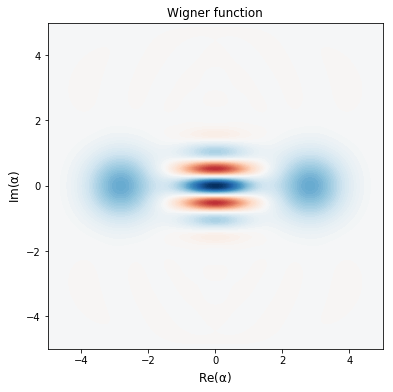
\includegraphics[width=0.45\textwidth]{figs/cat_0-no-trunc.png}
	}%
	\subcaptionbox{\(\ket{1_L}\) has two ``lobes'' along the imaginary axis.}{
		\centering
		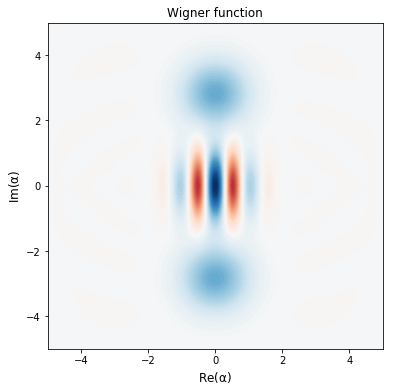
\includegraphics[width=0.45\textwidth]{figs/cat_1-no-trunc.png}
	}
	\caption{%
	Wigner function of the cat code logical basis states with \(\alpha = 2\).
	}%
	\label{fig:cat-code-basis-wigner}
\end{figure}

Before the encoding scheme for the cat code can be explained we will quickly need to review the theory behind qubits and resonators.

\subsection{Superconducting Resonators and Qubits}
Superconducting resonators are microwave resonators.
Although ideal harmonic resonators have equally spaced energy levels, in reality they are more or less anharmonic and the general Hamiltonian for a quantum anharmonic resonator is
\begin{equation}
    \Ham = \omega_{q} \au\ad + \frac{K_q}{2} (\au)^2\ad^2
    \label{eq:resonator-hamiltonian}
\end{equation}
where \( \omega \) is the resonance frequency, \( K \) is the anharmonic (self-Kerr) term and \(\ad\) is the annihilation operator which removes an excitation from the resonator.
Note that this is an approximate model as higher order terms have been neglected.

The anharmonicity can be visualized, see \Cref{fig:anharmonic-energies}, by plotting the eigenenergies of \Cref{eq:resonator-hamiltonian} as a function of \( K \).
A larger anharmonicity makes the energy spacing larger for excitation states higher than \(\ket{1}\).
This anharmonicity allows us treat the resonator as a qubit, by only driving at the frequency specified by the energy spacing between the first two states \( \ket{0} \) and \( \ket{1} \).
Throughout this thesis, the term ``qubit'' will be used to refer to an anharmonic resonator even though it has more than two energy levels.
Further note, the frequency corresponding to the energy spacing between the first two levels, will be referred to as \( \omega_{q} \), the ``resonance frequency of the qubit''.

\tikzfig{figs/energy-anharmonic}{The energy levels of a three-level resonator for anharmonicity \(K\in[0,1]\) and \(\omega=1\). A resonator has \(K~1\) while a qubit has \(K\neq0\).}{fig:anharmonic-energies}{25em}{20em}

Now if we couple a qubit to a resonator the Hamiltonian is
\begin{equation}
    \Ham(t) = \underbrace{\omega_{r}\au\ad + \frac{K_r}{2}(\au)^2\ad^2}_{\text{Resonator}} + \underbrace{\omega_{q}\bu\bd + \frac{K_q}{2}(\bu)^2\bd^2}_{\text{Qubit}} + \underbrace{g\qty(\au\bd+\ad\bu)}_{\text{Coupling}},
    \label{eq:hamiltonian-coupled}
\end{equation}
where \( \ad \) and \( \bd \) are the annihilation operators for the resonator and qubit respectively.
There is now a coupling term with coupling strength \(g\) which means that the resonator and the qubit can exchange excitations between each other.
\(g\) is assumed to be real for simplicity.
This is similar to the Jaynes-Cummings Hamiltonian, but now there are added self-Kerr (anharmonicity) terms for both the qubit and the resonator.
Another difference is that the Jaynes-Cummings model explicitly deals with a two-level qubit or atom, while this model has a ``qubit'' with arbitrary levels.
Note that the rotating wave approximation has been applied to the coupling term~\cite{wu_strong-coupling_2007}.

\subsection{Cat Code Encoding Scheme}
Now that we have an understanding of the coupled quantum system of interest we can understand how the cat code encoding scheme works.
In short, the quantum information of a superconducting qubit is carefully encoded into a cavity resonator by simultaneously driving the qubit and resonator system with microwave pulses.
To be specific, the unitary which we want to realise in a time \(T\) is
\begin{equation}
    \hat{U}(T) \qty(c_0\ket{0}+c_1\ket{0})\otimes\ket{0} = \ket{0}\otimes\qty(c_0\cat{}+c_1\cat[i]{})
    \label{eq:cat-code-unitary}
\end{equation}
where we see that the coefficients of an arbitrary qubit state are transferred to the resonator in the cat code basis.
Now the process of changing \Cref{eq:hamiltonian-coupled} to implement the transfer in \Cref{eq:cat-code-unitary} leads us to the theory of quantum optimal control.

\subsection{Quantum Optimal Control}
Quantum control is the process of controlling a quantum system by controlling the amplitude of a set of control operators~\cite{fisher_optimal_2010}.
Such a system can be described by a Hamiltonian of the following form~\cite{fisher_optimal_2010}
\begin{equation}
    \Ham(t) = \underbrace{\Ham_d}_{\text{Drift}} + \underbrace{u_0(t)\Ham_0 + \dotsc + u_N(t)\Ham_N}_{\text{Control}},
    \label{eq:optimal-control-hamiltonian}
\end{equation}
where in the cat code case \(\Ham_d\) is the Hamiltonian in \Cref{eq:hamiltonian-coupled}.
As these controls are usually electromagnetic pulses changing in time, they will be referred to as ``pulse shapes''~\cite{fisher_optimal_2010} in this thesis.

There are two main questions in quantum control: one of \emph{controllability} and one of \emph{optimal control}.
The first deals with the \emph{existence} of solutions given a Hamiltonian and the second with the \emph{optimized} solutions for the pulse shapes \(\qty{u_i(t)}\)~\cite{dalessandro_introduction_2007}.
The optimal solutions are generally not analytically solvable and thus the pulse shapes need to be discretized and numerically optimized in simulation.

~\citeauthor{ofek_extending_2016} numerically optimize their microwave pulse shapes using the GRAPE algorithm~\cite{khaneja_optimal_2005}. However, as there is no source code available for this implementation, this provides an opportunity to reproduce their result with an easy-to-use open source software package, and hopefully provide reference for future implementations.

\newpage
\section{Purpose of the Thesis}%
\label{sec:purpose}
The purpose of this thesis is to, as a proof of concept, numerically optimize microwave pulses to encode the quantum information of a qubit into a resonator in cat codes.
This is to provide future research with a boilerplate for performing encoding in cat codes.

The thesis is limited to
\begin{itemize}
    \item closed quantum systems without any interaction with the environment and
    \item only finding pulses that \emph{encode} the cat codes (no decoding).
\end{itemize}

\end{document}